\section{Results}
\label{sec:result}

For a CP-even Higgs boson, the mean value of Optimal Observable is expected to be 0 for both signal and background process. So a direct and totally model independent measurement of Higgs CP could be obtained from this with data. Table ~\ref{tab:meanOO} shows the observed mean Optimal Observable value in data and the statistical uncertainties. 

\begin{table}[]
\centering
\begin{tabular}{ll}
\hline
         & \textless{}OO\textgreater{} \\ \hline \hline
TT       &   $  0.014 \pm 4.004 $      \\ \hline
TL       &   $ -0.004 \pm 3.895 $      \\ \hline
LT       &   $ -0.013 \pm 3.752 $      \\ \hline
LL       &   $ -0.006 \pm 3.879 $      \\ \hline \hline
combined &                             \\ \hline
\end{tabular}
\caption{Mean values of Optimal Observable and statistical only uncertainty in 4 categories and their combination. }
\label{tab:meanOO}
\end{table}


A more precise measurement of CP-mixing parameter $\tilde{d}$ is performed with a maximum likelihood fit described in Section ~\ref{sec:fit}. The parameter of interest $\tilde{d}$ is scanned with step of 0.01 and other nuisance parameters are adjusted within their allowed constraints. Table ~\ref{tab:dtilde_mu_obs} summarized the best fit signal strength and $\tilde{d}$ with statistical and systematic uncertainty. Expected results from MC is shown in Table ~\ref{tab:dtilde_mu_exp}. \\

The expected and observed $\Delta NLL$ curve is shown in figure ~\ref{fig:NLLcurve} as a function of $~\tilde{d}$. In the expected result the signal strength is set to 1, and $\tilde{d}$ is set to 0, corresponding to the best estimate of sensitivity of the analysis based on SM prediction. The contribution from 4 categories are shown with statistical only $\Delta NLL$ curve in Figure ~\ref{fig:NLLcurve_4cate}. 

\begin{table}[]
\centering
\small
\begin{tabular}{lcccc}
\toprule
         & $\mu \pm unc.(stat.)$ &  $\tilde{d}\pm unc.(stat.)(68\% interval)$   & 95\% interval of $\tilde{d}$(stat.) & 95\% interval of $\tilde{d}$(stat.+syst.)  \\
\toprule
TT       &  $1.00\pm0.27 (0.25)$  &  $0.00^{+0.039(0.039)}_{-0.039(0.038)}$      &  $ [-0.092, 0.096] $                &  $ [-0.094, 0.099] $                       \\ \hline
TL       &  $1.00\pm0.36 (0.34)$  &  $0.00^{+0.062(0.061)}_{-0.062(0.061)}$      &  $ [-0.272, 0.254] $                &  $ [-0.295, 0.273] $                       \\ \hline
LT       &  $1.00\pm0.38 (0.35)$  &  $0.00^{+0.062(0.061)}_{-0.061(0.060)}$      &  $ [-0.303, 0.315] $                &  $ [-0.329, 0.337] $                       \\ \hline
LL       &  $1.00\pm1.12 (1.12)$  &  $0.00^{+1.407(1.197)}_{-1.293(1.148)}$      &  $ [-4.924, 5.071] $                &  $ [-5.551, 6.023] $                       \\
\bottomrule
combined &  $1.00\pm0.20 (0.17)$  &  $0.00^{+0.027(0.027)}_{-0.027(0.026)}$      &  $ [-0.057, 0.059] $                &  $ [-0.059, 0.060] $                       \\ 
\bottomrule
\end{tabular}
\caption{Expected results for signal strength and $\tilde{d}$. }
\label{tab:dtilde_mu_exp}
\end{table}

\begin{figure}[h]
  \centering
  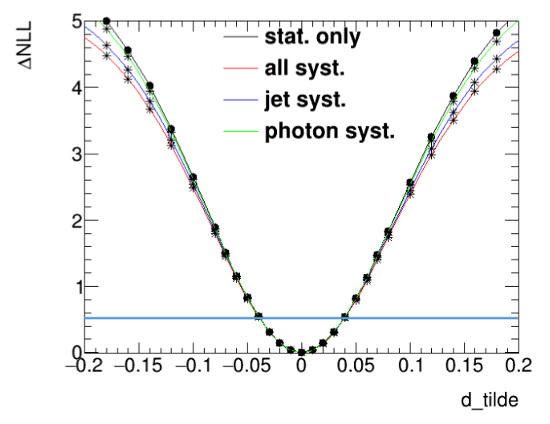
\includegraphics[width=.7\textwidth]{figure/NLLcurve.png}
  \caption{Expected $\Delta NLL$ curve for combined result. }
  \label{fig:NLLcurve}
\end{figure}

\begin{figure}[h]
  \centering
  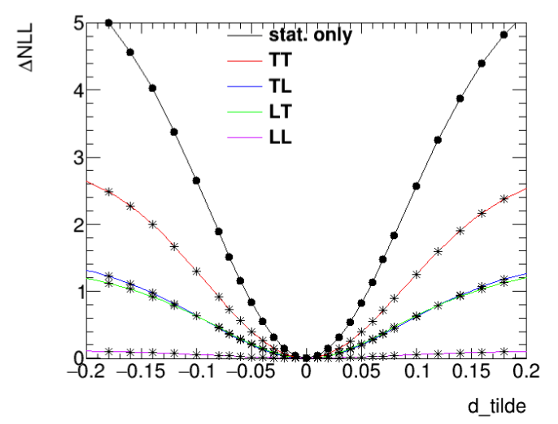
\includegraphics[width=.7\textwidth]{figure/NLLcurve_4cate.png}
  \caption{Statistical only $\Delta NLL$ curve for 4 categories. }
  \label{fig:NLLcurve_4cate}
\end{figure}



